\documentclass[tikz,border=6pt]{standalone}
\usepackage[utf8]{inputenc}
\usepackage{xcolor}
\usepackage{amsmath}
\usetikzlibrary{arrows.meta,calc,positioning,fit}
\renewcommand{\familydefault}{\sfdefault}

\definecolor{medBlue}    {HTML}{4A86B8}
\definecolor{baseGray}   {HTML}{9E9E9E}
\definecolor{vesselRed}  {HTML}{C0504D}
\definecolor{loss1}      {HTML}{F1D897}
\definecolor{panelGray}  {HTML}{CFCFCF}

\tikzset{
  font=\sffamily\footnotesize,
  arrow/.style={-{Latex[length=2.2mm,width=1.7mm]},draw=black,line width=1.0pt},
  panel/.style={rounded corners=8pt,draw=panelGray,dashed,line width=1.2pt,fill=white},
  model/.style={rectangle,rounded corners=3pt,draw=none,fill=medBlue,text=white,
    minimum width=4.0cm,minimum height=1.5cm,align=center,inner xsep=6pt,font=\bfseries\footnotesize},
  base/.style={rectangle,rounded corners=3pt,draw=none,fill=baseGray,text=white,
    minimum width=4.0cm,minimum height=1.5cm,align=center,inner xsep=6pt,font=\bfseries\footnotesize},
  data/.style={rectangle,rounded corners=3pt,draw=black!50,line width=0.9pt,fill=black!6,
    minimum width=4.2cm,minimum height=1.7cm,align=center,inner xsep=6pt,font=\scriptsize\itshape},
  mask/.style={rectangle,rounded corners=3pt,draw=none,fill=vesselRed,text=white,
    minimum width=5.2cm,minimum height=1.5cm,align=center,inner xsep=6pt,font=\bfseries\footnotesize},
  metricbox/.style={rectangle,draw=none,minimum width=5.4cm,minimum height=2.4cm,
    align=center,inner xsep=6pt,font=\bfseries\scriptsize},
  merge/.style={rectangle,rounded corners=3pt,fill=medBlue!18,draw=medBlue,line width=1.0pt,
    minimum width=5.4cm,minimum height=2.4cm,align=center,font=\bfseries\scriptsize,text=black},
  title/.style={font=\sffamily\bfseries\large,align=center},
}

\begin{document}
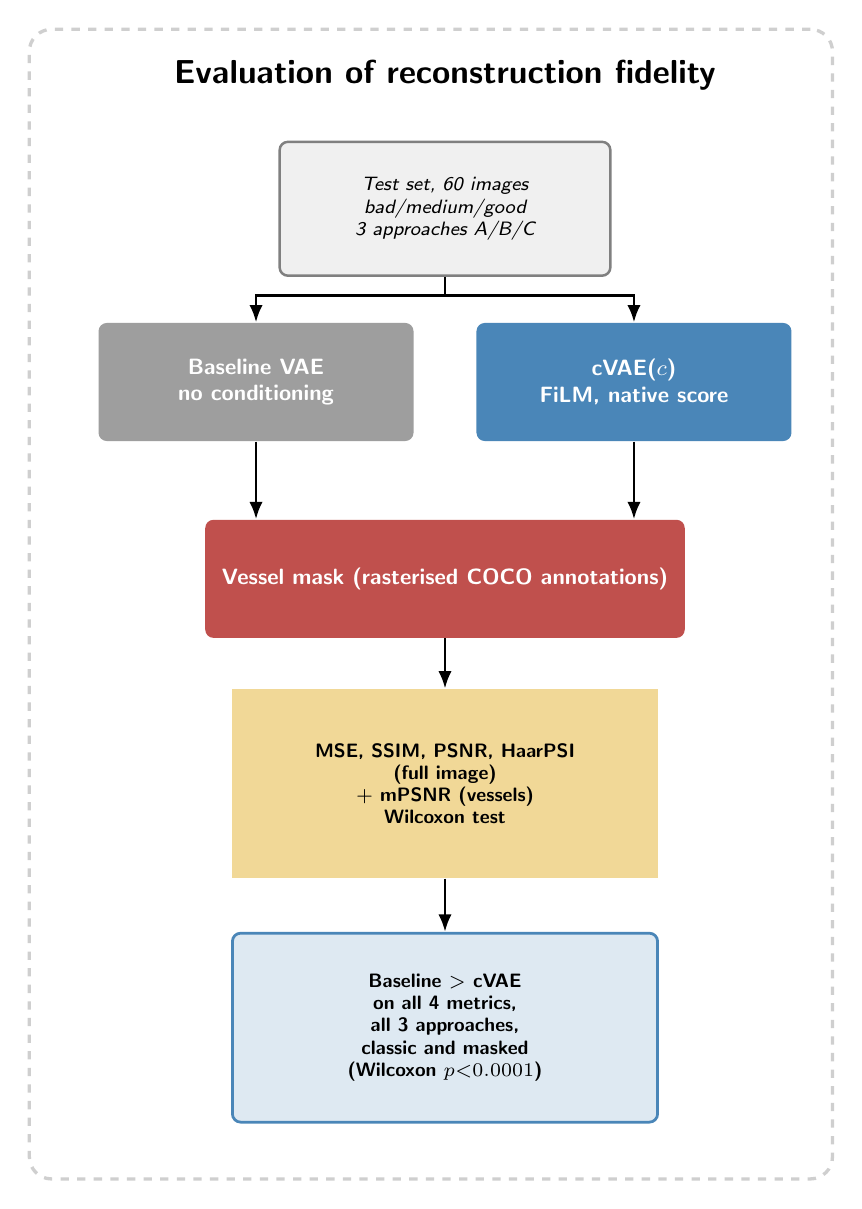
\begin{tikzpicture}[x=1cm,y=1cm]

\node[panel,minimum width=10.2cm,minimum height=14.6cm,anchor=north west] at (-.3,15.3){};

\node[title] at (5.0,14.7) {Evaluation of reconstruction fidelity};

\node[data] (testset) at (5.0,13.0) {Test set, 60 images\\bad/medium/good\\3 approaches A/B/C};

\node[base]  (basemodel) at (2.6,10.8) {Baseline VAE\\no conditioning};
\node[model] (cvaemodel) at (7.4,10.8) {cVAE($c$)\\FiLM, native score};

\draw[arrow] (testset.south) -- (5.0,11.9) -- (2.6,11.9) -- (basemodel.north);
\draw[arrow] (testset.south) -- (5.0,11.9) -- (7.4,11.9) -- (cvaemodel.north);

\node[mask] (mask) at (5.0,8.3) {Vessel mask (rasterised COCO annotations)};

\draw[arrow] (basemodel.south) -- (mask.north -| basemodel.south);
\draw[arrow] (cvaemodel.south) -- (mask.north -| cvaemodel.south);

\node[metricbox,fill=loss1] (metrics) at (5.0,5.7)
  {MSE, SSIM, PSNR, HaarPSI\\(full image)\\$+$ mPSNR (vessels)\\Wilcoxon test};

\draw[arrow] (mask.south) -- (metrics.north);

\node[merge] (concl) at (5.0,2.6)
  {Baseline $>$ cVAE\\on all 4 metrics,\\all 3 approaches,\\classic \emph{and} masked\\(Wilcoxon $p{<}0.0001$)};

\draw[arrow] (metrics.south) -- (concl.north);

\end{tikzpicture}
\end{document}
